\documentclass{article}
\usepackage{arxiv}
\usepackage[T1]{fontenc}
\usepackage[utf8]{inputenc}
\usepackage{amsmath,amssymb}
\usepackage{booktabs,tabularx,array}
\usepackage[numbers,sort&compress]{natbib}
\usepackage{microtype}
\usepackage{xcolor}
\usepackage{listings}
\usepackage{tikz}
\usetikzlibrary{arrows.meta,positioning}
\usepackage{url}
\usepackage[colorlinks=true,linkcolor=black,citecolor=black,urlcolor=blue!45!black]{hyperref}
\hypersetup{pdftitle={DLP Nova: A Reasoner with Geospatial and Temporal Extensions},pdfauthor={Raphael Volz}}
\renewcommand{\shorttitle}{DLP Nova: Geospatial and Temporal Extensions}
\renewcommand{\headeright}{Raphael Volz}
\renewcommand{\undertitle}{Systems paper draft}
\newcolumntype{Y}{>{\raggedright\arraybackslash}X}
\newcommand{\code}[1]{\texttt{#1}}
\lstset{basicstyle=\small\ttfamily,columns=fullflexible,keepspaces=true,
  breaklines=true,showstringspaces=false,frame=single,rulecolor=\color{black!20},
  xleftmargin=0.4em,xrightmargin=0.4em,aboveskip=0.8em,belowskip=0.8em}
\title{DLP Nova: A Reasoner with Geospatial and Temporal Extensions}
\author{Raphael Volz\\Pforzheim University}
\date{10 September 2026}

\begin{document}
\maketitle
\begin{abstract}
Ontology classification alone cannot determine whether a traffic sign is within
a geographic radius, whether a record was valid at an observation time, or how
a late event changes an observed geofence entry. These questions require
numerical computation and explicit policies for identity, time, source scope,
and incomplete external results. DLP Nova combines a Description Logic Programs
reasoner with a separately versioned rule-query language, checked temporal and
geospatial operations, finite provider scans, scoped minima, and event-window
state. It preserves the base ontology's open-world interpretation while
evaluating extensions over explicit finite snapshots. A shared native library
supports domain operations, resident point indexes, compiled Horn and local
query execution, and recoverable application sessions through C, Python, Swift,
and Kotlin interfaces. Executable examples cover calendar ages, time-dependent
traffic queries, bitemporal corrections, and late-event retractions. A focused
10,000-point experiment returns the same 11 radius answers after refining 13
indexed candidates rather than evaluating every point; build and query costs
are reported separately. Existing paired measurements additionally document
the benefit and upfront cost of retaining query preparation and minimum
supports. The contribution is an implemented integration with explicit semantic
and publication contracts, not a new temporal logic, a GeoSPARQL conformance
claim, or a general performance ranking.
\end{abstract}
\keywords{Description Logic Programs \and geospatial reasoning \and temporal reasoning
\and event windows \and native runtime \and ontology systems}

\section{Introduction}
Consider a vehicle application that needs to identify relevant stop signs near
its current observation. An ontology can infer that a particular category is a
subclass of \emph{StopSign}. Distance requires a coordinate system and metric;
validity requires a time interval; applicability may require explicit lane or
direction information. Replaying the same observation after a map correction
also requires knowing which map and recorded-time version the question refers
to. None of these choices follows from class membership alone.

Description Logic Programs (DLP) connect a restricted ontology language with
Horn-rule reasoning~\cite{grosof2003}. Volz's thesis developed this connection
into reasoning and maintenance services~\cite{volz2004}. DLP Nova builds on a
modern reconstruction of that base and adds an operational layer for questions
whose answers depend on explicit dates, geographic measurements, external
computations, or finite event histories. The name denotes the system described
here; its existing package and command names remain \code{dlp\_reasoner} and
\code{dlp}.

The engineering problem is more specific than adding a library call to a rule
body. A missing provider response must not become a negative answer. A minimum
over known child records must not become the historically first child without
a completeness premise. A point-index candidate must undergo exact distance
refinement. Expiration must retract results without erasing another surviving
support. A recovered application must not present results computed under an
incompatible map revision. These cases motivate a design in which meanings and
publication boundaries are explicit.

This paper makes three systems contributions. First, it presents the implemented
composition of a position-sensitive DLP compiler, finite rule-query language,
strict domains, providers, and windows. Second, it specifies the contracts that
govern metric and temporal interpretation, nonmonotonic answers, source
revisions, failure, and recovery across Python and native execution. Third, it
provides executable semantic cases and focused empirical evidence for selective
spatial access and repeated query preparation. The contribution is the concrete
integration and its inspectable behavior. The underlying DLP translation,
materialization methods, calendar calculations, and geodesic algorithms remain
attributable to prior work.

The companion paper \emph{Description Logic Programs Revisited} studies base
reasoning, maintenance, and comparisons with other reasoners~\cite{dlprevisited2026}.
The present paper is self-contained and concerns the extensions and application
runtime. Its measurements do not re-label the companion paper's ontology
benchmarks as geospatial or temporal evaluations.

\section{Base language and semantic boundary}
\label{sec:base}
The desktop authoring pipeline reads the thesis's concrete DLP syntax or an RDF
serialization of supported OWL axioms, translates the input into an RDF graph,
validates constructor positions, and compiles a Horn program. Unary predicates
represent class membership and binary predicates represent properties. Integrity
constraints have no ordinary conclusion. Auxiliary predicates factor compound
expressions; individual equality canonicalizes arguments with congruence.

\begin{table}[t]
\centering\small
\caption{Cumulative implementation modes. Constructor position remains part of
admissibility; this is a feature summary rather than an unrestricted grammar.}
\label{tab:profiles}
\begin{tabularx}{\linewidth}{lY}
\toprule
Mode & Principal additions \\
\midrule
L0 & Class/property inclusions and equivalences, intersections, union and
existential antecedents, universal consequents, has-value restrictions,
inverse/symmetric/transitive properties, domain and range. \\
L1 & Individual equality, functionality and inverse functionality, finite
enumeration antecedents, singleton consequents, top, and supported zero/one
cardinality forms. \\
L2 & Disjointness, complement constraints, bottom, maximum-zero restrictions,
explicit inequality, and \code{AllDifferent}. This is the desktop default. \\
L3 & Existential and positive minimum-cardinality consequents using Skolem
witnesses, with explicit distinctness for multiple required fillers. \\
\bottomrule
\end{tabularx}
\end{table}

Position is decisive. For example,
\begin{align*}
\exists\mathit{hasChild}.\mathit{Person}&\sqsubseteq\mathit{Parent}
&\text{compiles to }\quad
\mathit{Parent}(x)&\leftarrow\mathit{hasChild}(x,y),\mathit{Person}(y),
\end{align*}
which recognizes an existing filler and is admitted in L0. Reversing the
inclusion requires creating a witness and therefore needs L3. A universal
consequent only classifies existing property fillers; it does not generate an
edge. An equivalence must satisfy both inclusion directions. The historical
L0--L3 labels are implementation modes, not certificates of membership in
OWL 2 RL or another standardized profile~\cite{owlprofiles2012}.

The following concrete ontology illustrates an L0 classification and property
assertion. The keyword \code{partial} expresses a necessary superclass
condition, so the first statement entails that every stop sign is a traffic
sign.
\begin{lstlisting}
Namespace(ex = <https://example.org/nova#>)
Ontology(
  Class(ex:StopSign partial ex:TrafficSign)
  ObjectProperty(ex:locatedAt)
  Individual(ex:s1 type(ex:StopSign)
    value(ex:locatedAt ex:n1))
)
\end{lstlisting}

Failure to derive a fact means that it is not entailed, not that its negation is
entailed. Distinct IRIs need not denote distinct individuals. Explicit
disjointness and inequality can establish inconsistency, and an inconsistent
ontology is reported rather than exposed as an ordinary successful query
snapshot. Equality concerns individual arguments, not class/property predicate
identifiers. Unsupported axioms, including general disjunctive consequents,
universal antecedents, property chains, and maximum cardinalities above one,
fail explicitly.

L3 is not guaranteed to terminate: an axiom such as
$A\sqsubseteq\exists p.A$ may generate unbounded witnesses. The desktop engine
therefore bounds rounds, facts, and witness depth and distinguishes an
incomplete materialization from a completed one. The extension query runtime
requires a completed, consistent ontology snapshot. The base's datatype value
identity covers a stated subset, including supported strings, integer/decimal
values, and booleans; it does not implement full OWL datatype entailment or
arbitrary datatype ranges and facets. Explicit extension decoding of a date or
geometry does not expand that base entailment claim.

\section{Finite rule queries and system architecture}
\label{sec:architecture}
Figure~\ref{fig:architecture} separates ontology authoring, domain execution,
and application state. The extension language has a distinct \code{.dlq}
parser and begins with \code{version 1}. Its rules use positive relation atoms,
Boolean \code{filter} calls, scalar \code{bind} calls, finite provider
\code{scan} calls, and grouped \code{MIN}. Named \code{given} parameters make
query inputs and scope dependencies explicit. Extension results are separate
relations, not automatically asserted additions to the ontology closure.

\begin{figure}[t]
\centering
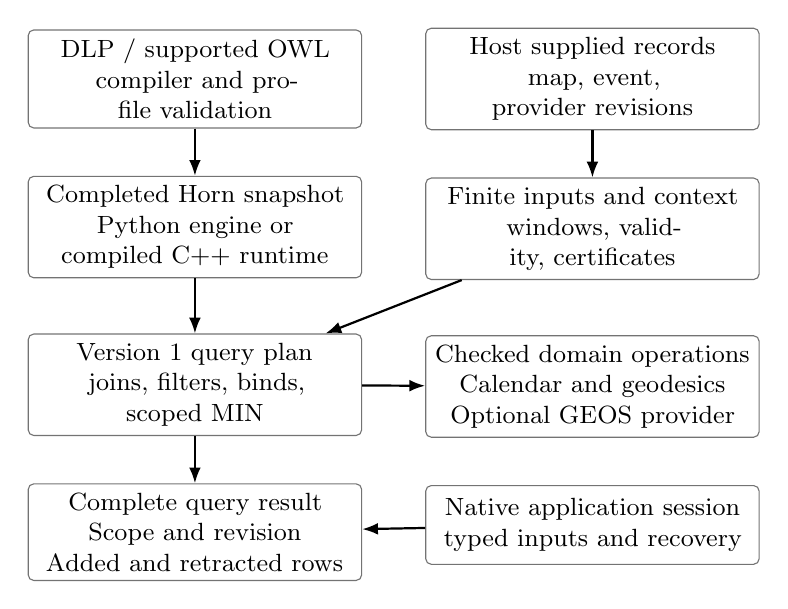
\begin{tikzpicture}[font=\small,
 box/.style={draw=black!55,rounded corners=2pt,align=center,minimum height=1cm,text width=4.0cm},
 arr/.style={-{Latex[length=2mm]},thick}]
\node[box] (author) {DLP / supported OWL\\compiler and profile validation};
\node[box,right=0.8cm of author] (external) {Host supplied records\\map, event, provider revisions};
\node[box,below=0.6cm of author] (horn) {Completed Horn snapshot\\Python engine or\\compiled C++ runtime};
\node[box,below=0.6cm of external] (context) {Finite inputs and context\\windows, validity, certificates};
\node[box,below=0.7cm of horn] (query) {Version 1 query plan\\joins, filters, binds, scoped MIN};
\node[box,below=0.7cm of context] (domain) {Checked domain operations\\Calendar and geodesics\\Optional GEOS provider};
\node[box,below=0.6cm of query] (result) {Complete query result\\Scope and revision\\Added and retracted rows};
\node[box,below=0.6cm of domain] (session) {Native application session\\typed inputs and recovery};
\draw[arr] (author) -- (horn);
\draw[arr] (external) -- (context);
\draw[arr] (horn) -- (query);
\draw[arr] (context) -- (query);
\draw[arr] (query) -- (domain);
\draw[arr] (query) -- (result);
\draw[arr] (session) -- (result);
\end{tikzpicture}
\caption{Logical responsibility boundaries. The diagram is not a promise that
every provider plan runs without a host: standalone native packages accept
local query plans, while provider transport and scoped source selection remain
host responsibilities.}
\label{fig:architecture}
\end{figure}

\subsection{Planning, binding, and termination}
An operation descriptor declares a URI, version, input and result types,
cardinality, and determinism. Planning checks descriptors and relation arities
without executing a domain operation or contacting a provider. It reorders body
nodes until their required inputs are bound, favoring ready filters before
unrelated joins. Every head variable must be supplied by a body node or a given
parameter. A scalar binding to an already bound variable checks agreement; it
does not overwrite the binding.

Positive recursion and pure Boolean filters are allowed. A dependency cycle
crossing a scalar bind, provider scan, aggregate, or non-pure filter is rejected.
An aggregate reads a completed lower stratum. This restriction prevents a
recursive arithmetic rule from generating an unbounded succession of values.
For a completed finite input, finitely many terminating operation calls, and
finite completed scans, each stratum consequently has a finite active domain:
positive recursive strata can add only finitely many ground tuples, while
value-producing steps occur above their inputs in the dependency order. This
is a conditional termination argument for the query layer. It does not prove
termination of an L3 ontology or of an arbitrary external function. Resource
exhaustion and interrupted providers are failed or incomplete evaluations.

\subsection{Three execution boundaries}
The Python \code{Reasoner} uses indexed semi-naive materialization. Choosing
\code{backend="native"} for this interface substitutes resident C++ relation
indexes while Python retains semantic orchestration, equality handling, and
maintenance control. This adapter is useful for maintaining desktop ontologies
without changing the authoring or reasoning API.

The separately compiled native Horn runtime is a different execution path. It
loads checked Horn input, implements equality and witness machinery in C++, and
uses indexed complete rule sweeps until a fixed point. It does not currently
port the Python semi-naive delta schedule or its DRed deletion algorithm.
Changed Horn inputs use its own reconstruction path. Calling both facilities
``native'' must therefore not imply identical algorithms or performance.

At the query layer, supported local plans can execute joins and typed scalar
operations in C++. The Python \code{QueryRuntime} still owns its input/output
and publication boundary; provider-dependent or unsupported custom operations
use the advertised host path. A compiled \code{.dlpn} package and native session
run the supported local Horn/query plan without CPython. Authoring, RDF
compilation, rule planning, accepted-record selection, provider transport, and
source-version policy are deployment responsibilities. This separation lets
mobile applications consume authored plans without shipping the Python toolchain.

\subsection{Query identity and publication}
An evaluation context identifies the ontology and equality revision, finite
input selection, query parameters, domain/operation versions, and provider
snapshots. A result is meaningful only under that context. The runtime publishes
immutable complete relations with scope/revision information and additions and
retractions from the preceding complete result. If a candidate fails, the old
complete result remains inspectable under its old revision while the current
evaluation is marked unsuccessful; it is not relabeled as the new answer.

Source guards, cancellation, deadlines, and provider revisions are checked even
on whole-answer cache hits. Cached scalar computations and prepared plans have
separate bounded lifetimes. A retained complete ontology snapshot and validated
query plan can survive changed query parameters. An ontology or equality change
invalidates dependent input selection. These checks matter for negative answers:
a cache of old successful witnesses cannot show that no newly added candidate
qualifies under a new map revision.

\section{Geospatial reasoning}
\label{sec:spatial}
\subsection{Metrics and typed geometry}
The baseline point type is WGS84 longitude/latitude in degrees, with longitude
first at the public boundary and explicit coordinate validation.
\code{sp:wgs84Distance} computes the shortest ellipsoidal surface distance in
metres using the bundled GeographicLib geodesic kernel, based on
Karney's algorithms~\cite{karney2013}. It ignores altitude and road topology.
\code{sp:dwithin} tests an inclusive radius against that metric. Both the Python
and native point-query paths use the same geodesic kernel; backend agreement
therefore tests integration and selection, not two independent geodesic algorithms.

An optional GEOS provider supports planar geometry operations. GEOS uses a
Cartesian model~\cite{geos}, so a projected coordinate system in metres can
support a planar metre distance, while longitude/latitude coordinates do not
automatically do so. The executable projected fixture uses EPSG:25832 and
distinguishes \emph{contains}, which excludes a point on a polygon boundary,
from \emph{covers}, which includes it. Its geometry snapshot records its CRS and
unit contract. A planar operation, a WGS84 geodesic, and a route length are
distinct computations.

These custom URIs do not claim the standard function namespace or conformance
classes of GeoSPARQL~\cite{geosparql11}. DLP Nova does not implement arbitrary
coordinate transformations or a complete GeoSPARQL query processor. GEOS is an
optional capability with separate packaging and licensing requirements; the
bundled point-distance capability does not require full GEOS or PROJ.

\subsection{Conservative candidates followed by exact refinement}
An immutable point index converts validated surface points to Earth-centered
Cartesian coordinates on the WGS84 ellipsoid and stores three sorted coordinate
columns. For query point $p$ and radius $r$, it searches the smallest axis
interval of the surrounding box and checks the remaining axes. To see why the
filter is conservative, let $X(p)$ be the Cartesian embedding and $d_g(p,q)$
the surface geodesic distance. Then
\[
  d_g(p,q)\leq r
  \quad\Longrightarrow\quad
  \|X(p)-X(q)\|_2\leq r
  \quad\Longrightarrow\quad
  |X_i(p)-X_i(q)|\leq r\quad(i=1,2,3).
\]
The chord cannot be longer than the surface path. Consequently, the box may
admit extra candidates but does not remove a true radius answer in exact
arithmetic. The implementation adds a one-micrometre padding for binary64
coordinate conversion and equivalent pole/wrap representations. Boundary,
antimeridian, and polar regressions test the numerical implementation; the
geometric implication alone is not a floating-point error proof.

The C++ index remains resident and returns bounded cursor batches. Every
candidate still undergoes the exact geodesic test $d_g\leq r$. A provider
descriptor marks the scan as a candidate superset, so its rows cannot be
presented as exact radius results before refinement. Index construction and
source validation are distinct costs from repeated querying.

\subsection{Combining classification, validity, and distance}
The following valid version-1 syntax illustrates the combination. The host
provides \code{ex:location} as accepted typed points,
\code{ex:validity} as finite start/end records, and a point-scan provider pinned
to \code{?snapshot}. The inferred \code{ex:StopSign} relation comes from the
completed ontology. All query parameters are explicit.
\begin{lstlisting}
version 1
prefix ex: <https://example.org/nova#>
prefix sp: <urn:dlp:spatial:>
prefix time: <urn:dlp:temporal:>

query near(?sign)
given (?position, ?radius, ?asOf, ?snapshot) :-
    scan sp:pointCandidates(?position, ?radius, ?snapshot) as ?sign,
    ex:StopSign(?sign),
    ex:location(?sign, ?point),
    ex:validity(?sign, ?start, ?end),
    bind time:interval(?start, ?end) as ?valid,
    filter time:contains(?valid, ?asOf),
    filter sp:dwithin(?position, ?point, ?radius).
\end{lstlisting}
This example is an integration pattern over supplied relations; it is not an
assertion that proximity establishes legal applicability. The traffic fixture
uses additional explicit road/lane relations when asking those questions. The
custom \code{time:} prefix above names DLP Nova operations, not OWL-Time.

\subsection{Map ingestion and routing boundaries}
The OSM store accepts bounded current snapshots and ordered changes, preserves
raw tags and ordered references, and validates that references resolve in the
final candidate snapshot. Typed node, way, and relation IDs have separate
spaces. Updates check versions, dependent geometry, tombstones, and resource
bounds before publishing a new snapshot. The optional PBF path uses a separately
installed reader. It is not an implicit network fetch or a claim that a supplied
extract is geographically complete.

\code{MapRuntime} constructs the candidate ontology closure before publishing
it with the map and point index. This supplies a consistent map/ontology revision
for queries. Current projections and indexes are conservatively rebuilt on
changed map snapshots; the implementation does not claim in-place regional
index maintenance. A failed candidate leaves the preceding publication available
under its original revision.

Routing uses a separate provider contract. A finite local directed graph can
minimize the sum of supplied nonnegative metre weights. An OSRM adapter instead
exposes the length of a fastest route under its configured profile. Unknown
coverage, known disconnection, provider failure, and a successful scalar value
are distinguishable outcomes. The local directed fixture and controlled HTTP
tests do not establish a deployed regional routing service, map matching, turn
restrictions, or traffic-sign applicability.

\section{Temporal operations, scoped minima, and event windows}
\label{sec:temporal}
\subsection{A deliberately bounded time profile}
The domain profile separates Gregorian dates, explicit-offset instants, local
times of day, fixed durations, and intervals. Instants and durations use signed
64-bit microseconds; serialized dates and timestamp years are restricted to
1--9999. Inputs finer than microsecond precision, leap seconds, timezone-less
instants, invalid dates, and unsupported calendar policies fail explicitly.
Named timezone conversion and a general calendar-month duration are outside
the implemented profile. The native date operations build on Hinnant's
\code{date}/\code{chrono} library~\cite{hinnantdate} behind the same checked domain ABI.

The operations include \code{before}, \code{after}, \code{equal}, fixed-duration
\code{add}, \code{elapsedSeconds}, \code{completedYears}, \code{interval},
\code{contains}, \code{intersects}, and \code{meets}. A proper interval has
same-type date or instant endpoints and strictly positive length. It denotes
$[a,b)$, so
\[
\operatorname{contains}([a,b),t)\iff a\leq t<b,
\qquad
\operatorname{intersects}([a,b),[c,d))\iff\max(a,c)<\min(b,d).
\]
Thus $[08{:}00,09{:}00)$ and $[09{:}00,10{:}00)$ meet without intersecting,
and only the second contains 09:00. An absent endpoint is not converted into
infinity. The bitemporal example uses a separate relation for an explicitly
open recorded-time interval.

Calendar age is computed as completed Gregorian years using an explicit
February-29 anniversary policy, such as March 1 in a common year. It is not
elapsed seconds divided by a nominal year length. Numeric operations keep
checked integers/exact decimals distinct from explicit binary64 conversion.
Division that cannot be represented within the exact decimal profile is an
error rather than an implicit approximation. The selected quantity operations
check units instead of silently adding metres to seconds.

\subsection{Validity and recorded time}
The history example separates the time at which a claim applies from the time
at which the record was accepted. At valid time 08:30, a selected speed limit
is 50 km/h when queried as recorded at 09:04:59, and 30 km/h as recorded at
09:05 after a correction. Both versions refer to the same valid interval
$[08{:}00,10{:}00)$. Rules bind proper intervals and check the two explicit
probe instants independently. These are finite historical snapshot queries,
not temporal-head rules or implicit clock advancement. The terminology is
compatible with OWL-Time's distinction between instants and intervals, but
the operations are not an implementation of the entire OWL-Time
ontology~\cite{owltime2017}.

\subsection{Minimum over accepted records}
The Bach extension asks for each parent's age at the earliest \emph{accepted
known} child's birth. It first validates and selects one normalized exact date
per person, exposing missing or conflicting claims as diagnostics. Taking the
minimum of conflicting birthdate claims would conceal a data-quality problem
rather than resolve it.

\begin{lstlisting}
version 1
prefix ex: <https://example.org/nova#>
prefix time: <urn:dlp:temporal:>
prefix policy: <urn:dlp:calendar-policy:>

query firstKnownDate(?parent, ?first) given (?scope, ?revision) :-
    MIN ?date GROUP_BY ?parent
    FROM ex:datedChild(?parent, ?child, ?date) AS ?first.

query ageKnown(?parent, ?child, ?age) given (?scope, ?revision) :-
    firstKnownDate(?parent, ?first),
    ex:datedChild(?parent, ?child, ?first),
    ex:acceptedBirthDate(?parent, ?birth),
    bind time:completedYears(?birth, ?first, policy:march1) as ?age.
\end{lstlisting}
The host has selected \code{ex:datedChild} for the declared scope/revision.
An empty group has no minimum. Joining the date back to its source retains all
tied children. Actual calendar policy values use the registry's declared policy
IRIs; the example uses its March-1 policy. Accepted date values are canonicalized
before the join. For arbitrary literal relations, equal decoded numeric values
can retain different RDF lexical identities, so value equality must be requested
explicitly where an identity join is insufficient.

For the repository's selected historical records, Johann Sebastian's known age
changes from 25 to 23 when the earlier child is inserted, and Maria Barbara's
from 26 to 24; removing those edges restores the previous values. These are
computations over an illustrative selected dataset, not claims to have
established a complete genealogy. The unqualified ``first child'' predicates
additionally require an explicit trusted completeness certificate binding the
parent-specific evidence, selection policy, scope, and revision. A completed
materialization proves that all rule consequences were computed for its input;
it does not prove completeness of that input about the world.

A bounded ordered support index retains eligible minimum groups between query
evaluations. Removing one of two tied supports preserves the minimum; removing
the last exposes the next value. Equality merges, splits, and source corrections
invalidate or update the relevant selections and supports. Upstream joins and
complete snapshot differencing still execute. This is limited aggregate-support
maintenance, not fully incremental evaluation of every query stratum.

\subsection{Explicit event-time state}
\code{WindowStore} and its C++ counterpart \code{NativeWindowStore} retain
identified events and expose a finite relation for
\[
W_e=\{\,v\mid e-w\leq\operatorname{time}(v)<e\,\},
\]
where the host supplies evaluation time $e$ and width $w$. Evaluation time and
watermark advance monotonically; the watermark cannot exceed the evaluation
time. Allowed lateness defines a rejection cutoff relative to the watermark.
No background clock or watermark generator is inferred from the ontology.
Advancing the clock expires rows even if no new event arrives.

Events carry stable IDs and increasing correction revisions. An identical
delivery retry is a no-op; distinct IDs preserve distinct observations even
when their values are equal. Changes to finalized old timestamps are rejected
under the configured lateness policy. The store retains the latest accepted
pre-window observation per key when requested, ordered by timestamp and event
ID. A missing predecessor remains unknown; it does not imply that the vehicle
was outside a fence.

Table~\ref{tab:entry} captures a consequence of this rule. Initially an outside
sample at second 00 precedes inside samples at 05 and 10. At evaluation time
12 the active interval is $[02,12)$. A late inside sample at 03 is accepted
under the fixture's declared policy. The observed entry moves from event05 to
event03, requiring both a retraction and an addition. This is a transition
between observations, not the exact physical crossing time. Advancing to
$[05,15)$ must retain the relevant predecessor knowledge so that event05 is
not incorrectly rediscovered as a new entry.

\begin{table}[t]
\centering\small
\caption{Executable late-event fixture; times are seconds after 08:00.
The sample at 00 is retained as predecessor history when outside the window.}
\label{tab:entry}
\begin{tabularx}{\linewidth}{lYY}
\toprule
State & Active event times & Entry consequence \\
\midrule
Before late delivery, $[02,12)$ & 05, 10 & event05 \\
After accepting event03 & 03, 05, 10 & retract event05; add event03 \\
Advance to $[05,15)$ & 05, 10 & no new entry at 05 \\
\bottomrule
\end{tabularx}
\end{table}

Window mutations publish immutable active/history differences and bound events,
keys, tombstones, offsets, and retained bytes. Native windows use a bounded
copy-and-validate update algorithm with retained-record scans; native residency
does not imply constant-time insertion. The rule language itself has no
\code{WINDOW}, \code{PREVIOUS}, \code{COUNT\_DISTINCT}, or \code{EMIT CHANGES}
syntax. Historical proposed files containing those forms are design material.
The executable host API supplies the active and predecessor relations to
ordinary finite queries.

\section{Updates, external results, and recoverable deployment}
\subsection{Support and external completeness}
The desktop base separates assertions from their consequences. Insertions
propagate deltas; eligible positive fact/rule deletions use delete-and-rederive
(DRed), an established materialized-view maintenance approach~\cite{gupta1993}.
Equality and existential retractions retain a reconstruction fallback. Aggregate
results and event transitions need their separate support and temporal contracts;
deleting an event must not automatically delete a fact that retains an ontology
or other-event support.

A provider snapshot identifies implementation, dataset, and relevant options,
including units, CRS, routing profile, or map revision. Requests carry correlated
row IDs and checked arguments. A finite scan becomes complete only when exhausted;
a page limit, interruption, or early cursor close is not proof of an empty
answer. Only complete successful results are eligible for memoization. Candidate
superset coverage additionally requires exact refinement.

The status distinction is essential. A successful Boolean false is a legitimate
value. A complete \code{NO\_ROUTE} result denotes a specific domain outcome.
\code{OUT\_OF\_REGION} is a coverage status and does not establish disconnection.
Unavailable service, malformed replies, changed snapshots, incomplete pages,
and deadlines prevent successful publication. The protocol checks these
conditions but relies on the adapter to honor the pinned snapshot; a revision
string alone cannot prove repeatable reads from a changing external service.

\subsection{Packages and native application sessions}
The desktop package format stores checked source and compiled records with
operation versions. The separate native \code{.dlpn} format contains typed
dictionaries, Horn/local-query IR, and provenance in bounded, checksummed,
length-delimited records. Loading validates references, arities, strata,
bindings, and capabilities before exposing an executable handle. Serialized
packages contain neither native pointers nor Python process hashes.

The native session facade owns a package, named parameters, and mutable
supplemental relations. Applications intern typed values or stable RDF identities,
replace or update a complete supplemental relation, execute, and page the result.
Failed input mutations preserve the previous input and answer. A successful
mutation advances the input revision and invalidates the old answer; a successful
run atomically publishes its complete result at that revision. An unsuccessful
run does not expose partial rows as an answer. Subsequent queries can reuse
prepared native rules, original Horn relations, and checked metadata.

One worker serializes session ownership, while cancellation has an explicit
cross-thread entry point. C, Python, Swift, and Kotlin/JNI bindings follow the
same underlying contract. The aggregate C++17 build supplies the baseline domain,
index, Horn, local-query, window, session, and recovery interfaces. The repository
records simulator/emulator application runs as well as native sanitizer checks;
these are deployment evidence for the tested targets, not physical-device
latency, battery, or memory-pressure measurements.

\subsection{Recovery and finite resource accounting}
Session checkpoints retain the checked package and explicit reachable inputs,
not current query results or execution cursors. Window checkpoints retain clocks,
event revisions, predecessor history, tombstones, source offsets, and policies.
An application recovery envelope binds the components to an exact external
context. Restoration validates all components and replay availability before
publishing the restored group; a fresh query execution is required. Source
gaps, incompatible context, or missing retained replay cannot be disguised as
successful continuity. Checksums detect accidental corruption and do not
authenticate a checkpoint.

Limits bound named stores, scanned rows/pages, caches, terms, and serialized
state. The limits are conservative accounting for those structures, not a bound
on total process RSS: old and candidate snapshots, indexes, exported results,
library allocations, and host memory can coexist. Applications must budget the
whole process and release old publications. This makes the tested resource
contract narrower and more actionable than claiming that an engine is simply
``mobile ready.''

\section{Evaluation and reproducibility}
\label{sec:evaluation}
The evaluation addresses three questions: do the combined operators produce the
intended finite answers and corrections; does a resident index reduce exact
distance work while preserving complete answers; and does retained preparation
help repeated queries with changed inputs? It combines executable fixtures,
focused differential regressions, a new point-index observation, and separately
preserved query-preparation measurements. It contains no comparative claim
against a dedicated geospatial database or temporal-logic reasoner.

\subsection{Executable semantic cases}
The Bach driver executes the actual parsed query file over accepted dates,
scoped minima, and calendar age. It checks the known-age answers 23 and 24
and the absence of complete-family answers without certificates. Separate
tests exercise update retractions, ties, empty groups, date conflicts,
earlier-child insertions, and equality merges/splits. The selected birthdate
normalization and source choices are recorded with the fixture; they are input
policies, not discoveries by the reasoner.

The traffic driver executes category inference, indexed candidate enumeration,
and WGS84 refinement. Its source fixture contains four radius and six distance
cases. The projected temporal/geographic driver checks validity endpoints,
planar distance, explicit lane selection, late-event entry correction, checkpoint
restoration, and idle expiry. Its history query separately checks the recorded-time
speed correction. Actual local Bach/history packages exercise the standalone
C++ query path; provider-driven geometry still requires host orchestration.

Python/native agreement is complemented by independent finite reference
calculations where available: set membership, completed calendar years, manually
specified expected answers, and exhaustive radius filtering. Randomized
maintenance tests compare updated minima and window histories with reference
states. This mixture tests more than scalar output parity. It still falls short
of a formal end-to-end proof, complete standards conformance, or field validation
of traffic decisions.

\subsection{Selective radius experiment}
The new \code{selective-radius-v1} run uses a deterministic $100\times100$ grid
of 10,000 WGS84 points and a 150-metre query radius. It verifies exact equality
of the complete indexed answer set with exhaustive evaluation using the same
GeographicLib kernel. On macOS 26.5.1 arm64, each path is evaluated five times;
Table~\ref{tab:spatial} reports medians and separate construction costs from
\path{benchmarks/dlp-nova-spatial-results.json}. All paths return 11 points.

\begin{table}[t]
\centering\small
\caption{New 10,000-point radius observation. Query times include obtaining the
complete radius result, not ontology compilation or materialization. The
exhaustive row reports warmed queries. A dash means no index construction.}
\label{tab:spatial}
\begin{tabular}{lrrrr}
\toprule
Path & Index build (ms) & Query median (ms) & Exact tests & Answers \\
\midrule
Exhaustive & --- & 110.487 & 10,000 & 11 \\
Python point index & 8.318 & 0.360 & 13 & 11 \\
Native point index & 29.564 & 0.164 & 13 & 11 \\
\bottomrule
\end{tabular}
\end{table}

The measured mechanism is the decrease from 10,000 exact evaluations to 13;
two candidates are rejected by refinement. Native domain loading costs
26.498 ms separately, and the first exhaustive query costs 132.692 ms.
Index construction is measured independently and is not amortized into the
query medians. The native index's higher build cost also illustrates why
construction and repeated-query boundaries matter.

This is one selective distribution, one radius, and one host. Paths execute in
fixed order in one process, rather than randomized isolated repetitions. The
shared exact kernel is an appropriate oracle for candidate recall but not an
independent check of geodesic numerical accuracy. The experiment measures the
point-index API with refinement, not a complete \code{.dlq} pipeline, network
ingestion, map changes, broad-radius workloads, or sustained event throughput.
The five observations are an engineering illustration with preserved raw
samples, not a basis for a general speedup factor or statistical population
claim.

\subsection{Repeated queries and minimum support reuse}
The separately retained \path{benchmarks/query-preparation-results.json}
compares the pre-optimization source at commit \code{521b82a} with recorded
later sources in alternating isolated Python processes. Five paired repetitions
use 500 base records and ten changing warm inputs per process. Whole-answer
caching is disabled; all first and warm complete answers are validated. Native
library loading/building, ontology construction, and independent answer checks
are outside the timed \code{evaluate()} calls. The artifact covers four workload
families; Table~\ref{tab:preparation} selects the two involving minima, including
the actual Bach query over explicitly synthetic child/date records.

\begin{table}[t]
\centering\small
\caption{Preserved paired preparation experiment, selected aggregate workloads.
Times are medians of per-process warm mean latencies. Ratios are medians of paired
speed ratios and need not equal the ratio of rounded displayed medians.}
\label{tab:preparation}
\begin{tabularx}{\linewidth}{Ylrrr}
\toprule
Workload & Backend & Before (ms) & After (ms) & Paired ratio \\
\midrule
One changed minimum group & Python & 34.685 & 19.976 & 1.75 \\
One changed minimum group & Native & 40.377 & 20.257 & 2.00 \\
Bach child-date correction & Python & 22.377 & 10.234 & 2.19 \\
Bach child-date correction & Native & 33.058 & 11.472 & 2.88 \\
\bottomrule
\end{tabularx}
\end{table}

The observations support reuse for these repeated-query workloads, with an
upfront tradeoff. Across all four families in that artifact, first-query latency
increased: Python ranges changed from 10.07--32.52 ms to 19.77--52.40 ms, and
native ranges from 29.44--41.53 ms to 38.87--51.05 ms. Preparing immutable
snapshots, accounting retained bytes, and constructing ordered supports costs
time before reuse becomes available. The native timings include the Python
\code{QueryRuntime} boundary and remain slower than Python in absolute time
on the displayed small workloads. They are not standalone native-session or
phone measurements. This experiment predates the new spatial run and is
reported with its own source/protocol record rather than presented as a new
rerun under the same environment.

\subsection{Artifacts and replication}
The repository contains source, example inputs, expected results, tests, and
benchmark runners. The manuscript's associated execution record is
\path{benchmarks/dlp-nova-example-results.json}; the separate build manifest records
source/evidence hashes for this draft. A local reproduction can execute:
\begin{lstlisting}
uv sync --extra dev --locked
uv run python examples/bach_temporal/run_queries.py --backend both
uv run python examples/traffic_signs/run_queries.py --backend both
# Requires the optional GEOS C library:
uv run python examples/temporal_geo/run_queries.py --backend both
uv run python -m benchmarks.extension_queries --side 100 --repeats 5 \
  --output /tmp/dlp-nova-spatial-results.json
\end{lstlisting}
The spatial runner may require a local C++17 compiler or the corresponding
precompiled library. These commands reproduce current-source observations;
the frozen query-preparation comparison must use its recorded source hashes
and baseline protocol for the original before/after claim. The manuscript
build compiles an independent PDF and source archive without altering the
earlier paper. No submission or publication status is implied by generating
those artifacts.

\section{Related work and limitations}
DLP Nova's ontology foundation follows the established DLP intersection of
ontology and rule languages~\cite{grosof2003,volz2004}; its L3 witness mode and
finite resource limits need their own scope statement. OWL 2 RL provides a
standard profile for rule-oriented ontology reasoning~\cite{owlprofiles2012}.
The historical modes here are not substitutes for checking that standard's
grammar and semantics. The companion study evaluates the base reasoner's
specializations; its findings do not establish the originality or efficiency
of these domain extensions~\cite{dlprevisited2026}.

RDFox also combines Datalog materialization with filters, binds, stratified
aggregation, and date/time and geospatial functions~\cite{rdfoxreasoning,rdfoxquerying}.
Combining rules with temporal or spatial calculations is therefore not, by
itself, a novelty claim.

GeoSPARQL defines a geographic vocabulary and query-language extensions with
specified conformance classes~\cite{geosparql11}. DLP Nova instead exposes a
bounded custom rule/operator contract with a point-distance baseline and an
optional planar geometry provider. GeographicLib and GEOS supply mature
numerical geometry machinery~\cite{karney2013,geos}; using those libraries is
an implementation choice rather than a new geodesic or topology algorithm.
OWL-Time provides a vocabulary for temporal entities and
relations~\cite{owltime2017}. Representing that vocabulary does not itself
supply an event scheduler or finite-source completeness policy.

LARS gives a formal framework for reasoning over streams with window
operators~\cite{lars2018}. DLP Nova's current interface materializes explicit
host-controlled finite windows and does not implement the full LARS language
or answer-set semantics. MeTeoR implements reasoning in DatalogMTL with metric
temporal operators~\cite{meteor2025}. DLP Nova does not claim those operators,
its temporal entailment guarantees, or continuous-time interval propagation.
Ordering two timestamps or querying finite validity intervals is a narrower
capability than metric temporal logic reasoning.

Future extensions should be grounded in requirements from concrete applications
or users. The Bach, traffic-sign, and event-window examples establish executable
workflows; they do not establish demand for additional language or domain
features. A proposed extension should begin with an application dataset,
question, or update sequence that the current implementation cannot adequately
handle, together with an observable acceptance criterion. This establishes
whether the relevant gap concerns expressivity, interoperability, data coverage,
or measured resource use before an implementation is selected.

Present limitations remain material to that assessment. Providers must honor
their revision contracts, and applications must establish the legitimacy of
accepted records and trusted completeness certificates. Map publication
currently rebuilds closure/index state, upstream aggregate joins are not fully
incremental, and native windows scan retained records during transactions.
Their practical importance should be evaluated using the identified
application's data volumes, event ordering, and update patterns, reporting
retained memory and ingestion-to-answer latency with complete-answer checks.
Physical-device lifecycle, energy, and memory-pressure qualification remains
separate from simulator/emulator execution and is needed when the intended
deployment requires evidence on those devices.

\section{Conclusion}
DLP Nova demonstrates an executable way to combine restricted ontology
reasoning with geospatial computation, temporal selection, scoped aggregates,
and finite event histories. Its central design decision is to make metric,
time, identity, source scope, and complete-result publication explicit at every
boundary. That decision supports interpretable failures and recoverable native
applications while preserving the base ontology's open-world semantics.
The available evidence establishes the worked answers, update behaviors, and
selected benefits of resident state; it also exposes construction costs and
current scalability limits. The result is a concrete systems contribution
whose supported behavior can be exercised and extended without assuming a
new temporal logic or universal performance advantage.

\bibliographystyle{plainnat}
\bibliography{dlp-nova-references}
\end{document}
